\documentclass[a4paper]{IEEEtran}

\usepackage[ngerman]{babel}
\usepackage[utf8]{inputenc}
\usepackage{amssymb}
\usepackage[T1]{fontenc}
\usepackage[per-mode=fraction]{siunitx}
\usepackage{graphicx}

\usepackage{amsmath}

\newcommand{\eqname}[1]{\tag*{#1}}% Tag equation with name
\newenvironment{conditions}
  {\par\vspace{\abovedisplayskip}\noindent\begin{tabular}{>{$}l<{$} @{${}={}$} l}}
  {\end{tabular}\par\vspace{\belowdisplayskip}}

\title{Formelsammlung Physik}
\date{6. November 2019}
\author{Damien Flury}

\begin{document}
  \maketitle
  \section{Einheiten}
  \subsection{SI-Basiseinheiten}
    \begin{tabular}{|l|l|c|}
      \hline
      \textbf{Physikalische Grösse} & \textbf{Einheit} & \textbf{Symbol} \\ \hline \hline
      Länge & Meter & m \\
      Zeit & Sekunde & s \\
      Masse & Kilogramm & kg \\
      Temperatur & Kelvin & K \\
      Stromstärke & Ampère & A \\
      Stoffmenge & Mol & mol \\
      Lichtstärke & Candela & cd \\
      \hline
    \end{tabular}
  \subsection{Umrechnung}
  \begin{align}
    1 \si{\metre\per\second} &= 3.6 \si{\kilo\metre\per\hour}\\
    1 \si{\bar} &= 10^5 \si{\pascal} \\
  \end{align}
  \section{Kinematik}
  \subsection{Translation (geradlinige Bewegung)}
  \subsubsection{Gleichförmige Translation}
  \begin{align}
    v &= \lim_{t \to 0} \frac{\Delta{}s}{\Delta{}t} \\
    s &= v \cdot t + s_0
  \end{align}
  \subsubsection{Gleichförmig beschleunigte Translation}
  \begin{align}
    a &= \lim_{t \to 0} \frac{\Delta{}v}{\Delta{}t} \\
    v_2{}^2 - v_1{}^2 &= 2 \cdot a \cdot s \\
    s &= \frac{1}{2} \cdot v \cdot t \\
    s &= \frac{1}{2} \cdot a \cdot t^2 \\
    s = \frac{v_1 + v_2}{2} \cdot t &= v_1 \cdot t + \frac{1}{2} \cdot a \cdot t^2 = \frac{v_2{}^{2} - v_1{}^2}{2 \cdot a}
  \end{align}
  \subsection{Kreisbewegung}
  \begin{equation}
    \tau = \frac{1}{n}
  \end{equation}
  \begin{conditions}
    \tau & Periodendauer \\
    n & Umlaufzeit
  \end{conditions}

  \section{Dynamik}
  Grundgesetz der Dynamik:
  \begin{equation}
    F = m \cdot a
  \end{equation}
  \begin{equation}
    [F] = \si{\newton} = \si{\kilo\gram} \cdot \si{\metre\per\second\squared}
  \end{equation}

  \subsection{Reibung}

  \subsubsection{Schiefe Bahn}

  \begin{center}
    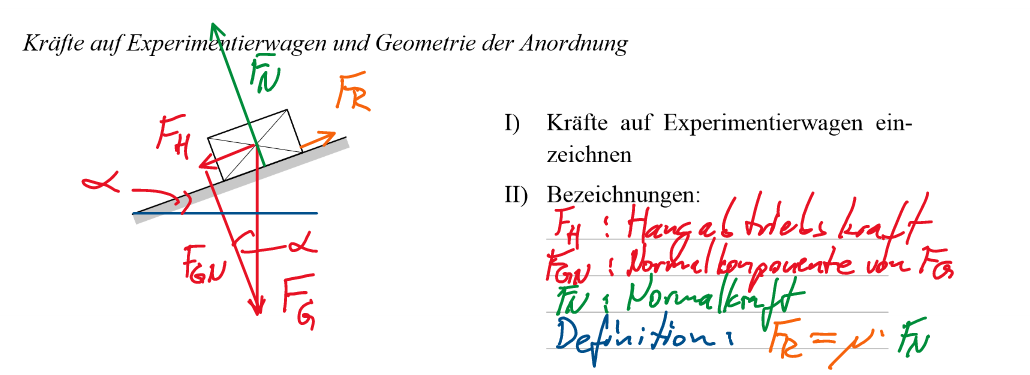
\includegraphics[width=8cm]{images/dynamik_schiefe_bahn.png}
  \end{center}
  \begin{equation}
    F_R = \mu \cdot F_N
  \end{equation}
  \begin{equation}
    F_H = F_G \cdot \sin{\alpha}
  \end{equation}
  \begin{equation}
    F_N = F_{GN} = F_{G} \cdot \cos{\alpha}
  \end{equation}
  Resultierende Kraft:
  \begin{align}
    F_a &= F_H - F_R \\
    F_a &= F_G \cdot (\sin{\alpha} - \mu \cdot \cos{\alpha})
  \end{align}
  Daraus folgt bei a = 0:
  \begin{equation}
    \mu = \tan{\alpha}
  \end{equation}


  \subsubsection{Dichte}
  \begin{equation}
    \rho = \frac{m}{V}
  \end{equation}
  \begin{equation}
    [\rho] = \frac{kg}{m^3}
  \end{equation}

  \section{Arbeit, Energie, Leistung, Wirkungsgrad}
  \begin{equation}
    W = F \cdot s
  \end{equation}
  \begin{equation}
    [W] = N \cdot m = J
  \end{equation}

  \subsection{Hub- und Verschiebearbeit}
  \subsubsection{Hubarbeit}
  \begin{equation}
    W = m \cdot g \cdot h = F_G \cdot h
  \end{equation}
  \subsubsection{Verschiebearbeit}
  \begin{equation}
    W = F_R \cdot s
  \end{equation}

  \subsection{Feder}
  \begin{center}
    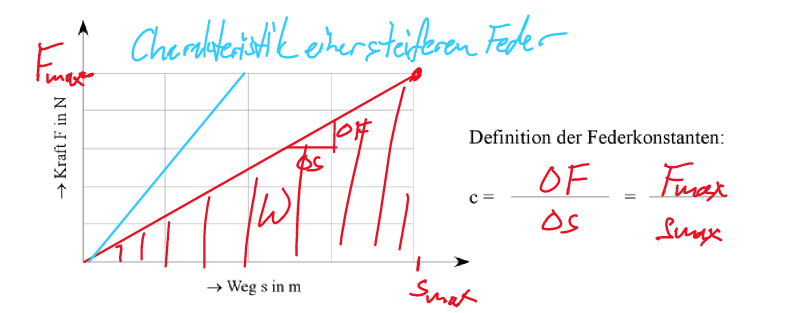
\includegraphics[width=8cm]{images/spring.png}
  \end{center}

  \begin{equation}
    c = \frac{\Delta F}{\Delta s} = \frac{F_{max}}{s_{max}}
  \end{equation}
  
  \subsubsection{Federspannungsarbeit}
  \begin{equation}
    W = \frac{1}{2} \cdot F \cdot s = \frac{1}{2} \cdot c \cdot s^2
  \end{equation}
  
  \subsection{Beschleunigungsarbeit}
  \begin{equation}
    W = \frac{1}{2} \cdot m \cdot v^2
  \end{equation}

  \subsection{Leistung}
  \begin{equation}
    P = v \cdot F
  \end{equation}

  \section{Statik}
  \subsection{Drehmoment}
  \begin{equation}
    \vec{M} = \vec{r} \times \vec{F}
  \end{equation}
  \subsubsection{Bei rechtem Winkel}
  \begin{equation}
    M = r \cdot F
  \end{equation}
  \begin{equation}
    P = v \cdot \frac{M}{r}
  \end{equation}

  \section{Hydrostatik}
  \subsection{Druck}
  \begin{align}
    p &= \frac{F}{A} \\
    [p] &= Pa
  \end{align}
  \begin{equation}
    p = \rho \cdot g \cdot h
  \end{equation}
  
  \subsubsection{Kolben}
  \begin{equation}
    \frac{F_1}{F_2} = \frac{A_1}{A_2} = \frac{{d_1}^2}{{d_2}^2}    
  \end{equation}
  \begin{equation}
    A_1 \cdot s_1 = A_2 \cdot s_2
  \end{equation}
  \begin{equation}
    W_1 = W_2 \Rightarrow F_1 \cdot s_1 = F_2 \cdot s_2
  \end{equation}
  \begin{equation}
    \frac{s_1}{s_2} = \frac{F_2}{F_1} = \frac{A_2}{A_1} 
  \end{equation}

  \section{Taschenrechner}
  \subsection{Stunden zu Stunden, Minuten and Sekunden konvertieren}
  \begin{equation}
    Zeit \blacktriangleright \mbox{DMS}
  \end{equation}

  \section{Konstanten}
  \begin{equation}
    g = 9.81 \si{\metre\per\square\second}
  \end{equation}
\end{document}